%!TEX program = xelatex
\documentclass[11pt, a4paper, titlepage]{article}

\usepackage{amsmath}
\usepackage{amssymb}
\usepackage{multirow}

% fonts
% \usepackage{xeCJK}
% \setCJKmainfont[BoldFont=SimHei]{SimSun}
% \setCJKfamilyfont{hei}{SimHei}
% \setCJKfamilyfont{kai}{KaiTi}
% \setCJKfamilyfont{fang}{FangSong}
% \newcommand{\hei}{\CJKfamily{hei}}
% \newcommand{\kai}{\CJKfamily{kai}}
% \newcommand{\fang}{\CJKfamily{fang}}
%
\usepackage[UTF8,heading=false,scheme=plain]{ctex}
% style
\usepackage[top=2.54cm, bottom=2.54cm, left=3.18cm, right=3.18cm]{geometry}
\linespread{1.5}
\usepackage{indentfirst}
\parindent 2em
\punctstyle{quanjiao}
\renewcommand{\today}{\number\year 年 \number\month 月 \number\day 日}

% figures and tables
\usepackage{graphicx}
\usepackage{longtable}
\usepackage[font={bf, footnotesize}, textfont=md]{caption}
\makeatletter
    \newcommand\fcaption{\def\@captype{figure}\caption}
    \newcommand\tcaption{\def\@captype{table}\caption}
\makeatother
\usepackage{booktabs}
\renewcommand\figurename{图}
\renewcommand\tablename{表}
\newcommand{\fref}[1]{\textbf{图 \ref{#1}}}
\newcommand{\tref}[1]{\textbf{表 \ref{#1}}}
\newcommand{\tabincell}[2]{\begin{tabular}{@{}#1@{}}#2\end{tabular}} % multiply lines in one grid

\usepackage{listings}
\lstset{basicstyle=\ttfamily}

\usepackage{xcolor}
\renewcommand{\r}{\color{red}}
\usepackage{tabulary}
\usepackage{url}
\usepackage{hyperref}

% start of document
\title{\textbf{DC\_Online \\ 数字电路在线实验平台二期工程 \\ 设计说明文档}}

\author{
    丁雨晖 \quad 计54 \quad 2015010866 \\
    祝方韦 \quad 计54 \quad 2015011317 \\
    梁宸 \quad \quad 计54 \quad 2015011325 \\
    蔡坤泰 \quad 计55 \quad 2015011809
}
\date{\today}

% -----------------start here------------------%
\begin{document}

\maketitle

\newpage
\tableofcontents
\newpage

\section{项目概述}
\section{数据库}
我们使用Mongodb作为服务器端使用的数据库,并使用Mongodb的ORM框架Mongoose来管理数据库,Mongodb是非关系型的数据库,但为了便于理解,在说明的时候借鉴了关系型数据库的相关概念。

我们设计的数据库共分为user,example,homework,project,message和submit六个部分,下面分别进行具体说明。Mongodb会为每一条记录赋予一个“\_id”域作为主键,在下面的表格中省略。


User表存储所有用户的信息。用户的用户名userName保证唯一。projectBox与homeworkBox中的元素为project记录的“\_id”,通过“\_id”可以到project表中查询到对应的project记录的详细信息。authority域为0表示普通用户,为1表示用户具有管理员权限。
\begin{center}
	\begin{longtable}{p{0.25\columnwidth}p{0.15\columnwidth}p{0.4\columnwidth}}
		\toprule
		 域名 & 类型 & 描述 \\
		 \midrule
		 userName & String & 用户名 \\
		 password & String & 密码 \\
		 uniquetoken & String & 用于标识当前在线用户的令牌 \\
		 authority & Number & 用户权限 \\
		 group & String & 用户所属分组 \\
		 ifaccounts9 & Number & 是否通过accounts9账号登陆 \\
		 projectBox & Array & 自定义项目列表 \\
		 homeworkBox & Array & 学生作业列表 \\
		 \bottomrule
	\end{longtable}
	\tcaption{User}
\end{center}


Project表记录了所有用户自定义项目(不包括管理员创建的样例)以及作业实例的详细信息。管理员布置作业以后,系统会在数据库的Homework表中添加一条作业记录,同时会在Project表中为每位学生生成一个作业实例,这样学生登陆后会在主页上看到一个空的作业项目,便可以开始进行操作。简单来说,Homework记录与Project记录为抽象与实例的关系。需要注意的是,Mongodb不要求Schema中的每一个域都在一条记录中出现,这为我们的实现带来了方便。如果一个Project记录的is\_homework为真,则意味着它为一个作业实例,这时这条记录中会出现homework域,score域以及hwSubmitBox域,而不会出现submitBox域;反之。

无论是普通项目还是作业实例,其余的域的意义都是相同的。type域为0表示该项目为拖拽项目,为1则表示该项目为文本编辑器项目。compileStatus用一个数字来表示当前该项目的编译状态:0表示上次编译是成功的;1表示还没有进行过任何编译;2表示曾经编译成功,但是上一次编译失败;3表示历次编译都失败了。
\begin{center}
	\begin{longtable}{p{0.25\columnwidth}p{0.15\columnwidth}p{0.4\columnwidth}}
		\toprule
		 域名 & 类型 & 描述 \\
		 \midrule
		 projectName & String & 项目名称 \\
		 author & ObjectId & 作者 \\
		 type & Number & 项目类别 \\
		 deleted & Boolean & 项目是否已被删除 \\
		 createTime & Date & 项目创建时间 \\
		 lastModifiedTime & Date & 上次修改时间 \\
		 filePath & String & 项目文件路径 \\
		 inputFile & String & 项目激励文件名 \\
		 submitBox & Array & 提交列表(自定义项目) \\ 
		 compileStatus & Number & 编译状态 \\ 
		 topEntityName & String & 顶层实体名称 \\
		 is\_homework & Boolean & 该项目是否是布置的作业 \\
		 homework & ObjectId & 项目对应于哪个布置的作业 \\
		 score & Number & 作业得分 \\
		 hwSubmitBox & Array & 作业提交列表 \\ 
		 input & Array & 输入端口 \\ 
		 output & Array & 输出端口 \\
 		 lastSimulationTime & Number & 上次仿真时间 \\
		 \bottomrule
	\end{longtable}
	\tcaption{Project}
\end{center}


Example表存储了管理员创建的样例信息。Example记录的内容与Project记录的内容是差不多的,但对二者的操作不同,同时也为了方便数据库的管理,因此将样例与一般的项目信息分别存储。
\begin{center}
	\begin{longtable}{p{0.25\columnwidth}p{0.15\columnwidth}p{0.4\columnwidth}}
		\toprule
		 域名 & 类型 & 描述 \\
		 \midrule
		 projectName & String & 样例名称 \\
		 author & ObjectId & 样例作者 \\
		 type & Number & 样例类别 \\
		 deleted & Boolean & 样例是否已被删除 \\
		 createTime & Date & 样例创建时间 \\
		 lastModifiedTime & Date & 上次修改时间 \\
		 filePath & String & 样例文件路径 \\
		 inputFile & String & 样例激励文件名 \\
		 submitBox & Array & 提交列表 \\ 
		 compileStatus & Number & 编译状态 \\ 
		 topEntityName & String & 顶层实体名称 \\
		 ifvisibletoUser & Boolean & 样例是否对用户可见 \\
		 isHomework & Boolean & 样例是否被作为作业发布 \\
		 input & Array & 输入端口 \\ 
		 output & Array & 输出端口 \\
 		 lastSimulationTime & Number & 上次仿真时间 \\
		 \bottomrule
	\end{longtable}
	\tcaption{Example}
\end{center}

Homework表存储了管理员发布的作业信息。每个发布的作业都必须与已有的一条Example记录相关联,relateExample域即表示关联的Example记录的“\_id”,correspondProject数组中的元素即为这条作业记录所对应的全部作业实例。由于Homework记录与Example记录相关联,因此Homework记录中无需保存作业的类型(拖拽或文本编辑)及输入输出端口名等信息,直接在Example表中查询即可。
\begin{center}
	\begin{longtable}{p{0.25\columnwidth}p{0.15\columnwidth}p{0.4\columnwidth}}
		\toprule
		 域名 & 类型 & 描述 \\
		 \midrule
		 relateExample & ObjectId & 与此作业关联的样例 \\
		 homeworkName & String & 作业名称 \\
		 describe & String & 作业描述 \\
		 deadline & Date & 作业提交截止日期 \\
		 totalsimfiles & Number & 标准测评文件数目 \\
		 author & ObjectId & 作业的布置者 \\
		 correspondProject & Array & 与此作业关联的作业实例 \\
		 \bottomrule
	\end{longtable}
	\tcaption{Homework}
\end{center}

Message表存储了管理员发布的课程公告,对所有学生可见,为了便于操作将这些信息单独用一张表存储。
\begin{center}
	\begin{longtable}{p{0.25\columnwidth}p{0.15\columnwidth}p{0.4\columnwidth}}
		\toprule
		 域名 & 类型 & 描述 \\
		 \midrule
		 author & ObjectId & 公告的发布者 \\
		 createTime & Date & 公告发布时间 \\
		 title & String & 公告的标题 \\
 		 content & String & 公告的内容 \\
		 \bottomrule
	\end{longtable}
	\tcaption{Message}
\end{center}

Submit表中的一条记录对应于一次提交(样例,普通项目或是作业实例),因为对Submit记录的访问均通过项目记录,不会直接对Submit表进行操作,因此将所有类型的Submit记录统一存储不会造成混乱。其中一些域的含义会在之后详细说明。
\begin{center}
	\begin{longtable}{p{0.25\columnwidth}p{0.15\columnwidth}p{0.4\columnwidth}}
		\toprule
		 域名 & 类型 & 描述 \\
		 \midrule
		 time & Date & 提交时间 \\
		 project & ObjectId & 所属的项目 \\
		 state & Number & 表示仿真是否完成 \\
		 stdMsg & String & 编译仿真的标准输出 \\
		 errMsg & String & 编译仿真的错误信息 \\
		 filePath & String & 本次提交对应的文件路径 \\
		 inputFile & String & 本次提交对应的激励文件名 \\
		 simulateRes & String & 仿真结果文件名 \\
		 \hline
		 xtime & String & \multirow{4}*{用于测评的参数} \\
		 lastlist & Array & ~ \\
		 changelist & Array & ~ \\
		 signalname & Array & ~ \\
		 \hline
		 score & Number & 本次提交得分 \\
		 simulationTime & Number & 仿真次数 \\
		 \bottomrule
	\end{longtable}
	\tcaption{Submit}
\end{center}

\section{编译仿真与前端仿真}

本部分主要说明本组项目中后端modelsim编译仿真与前端实时仿真模块实现的细节。


编译仿真:

我们通过脚本调用modelsim进行vhdl文件的编译仿真。脚本文件位于public/files中,文件名为model.sh,相关的modelsim编译与仿真命令如下:

\begin{table}[h!]
\centering  
\caption{modelsim编译仿真命令}  
\begin{tabular}  
{>{\columncolor{white}}rc}  
\toprule[1pt]  
\rowcolor[gray]{0.9} 命令    &描述\\  
\midrule  
{filename=param1 \\ jiliname=param2 }   &\multicolumn{1}{>{\columncolor{white}[0pt][0pt]}c}{vhdl源文件名和激励文件文件名分别 为参数1和参数2 } \\

vlib -unix work &\multicolumn{1}{>{\columncolor{white}[0pt][0pt]}c}{创建工作库work}   \\  
vcom filename.vhd jiliname.vhd   &\multicolumn{1}{>{\columncolor{white}[0pt][0pt]}c}{编译源文件和激励文件 }    \\ 
vsim -c -do "vcd add wave /\$\{jiliname\}/*" -do "run 3000ns" -do "quit -sim" -do "q" \$\{jiliname\}   &\multicolumn{1}{>{\columncolor{white}[0pt][0pt]}c}{通过激励文件对源文件进行仿真,仿真时间3000ns} 
\bottomrule[1pt]  
\end{tabular}  
\end{table}  

vcd文件解析

modelsim仿真会生成.wlf文件,通过脚本文件可以将.wlf文件转化为通用 的.vcd文件。为了了生成波形图形所需的数据,我们需要对.vcd文件进行解 析。我们使用node.js中的Duplex流对文件进行了处理。主要函数列表如下: 

\begin{table}[h!]
\centering  
\caption{modelsim编译仿真命令}  
\begin{tabular}  
{>{\columncolor{white}}rcc}  
\toprule[1pt]  
\rowcolor[gray]{0.9} 函数名称    &说明 &返回值\\  
\midrule  
state (initial, props)   &\multicolumn{1}{>{\columncolor{white}[0pt][0pt]}c}{将.vcd 文件分为不同的部 分,将文件的每一行标注为不同的状态(是否为波形数据、是否是仿真时间)}  &{该行文件的状态}\\

vcdStream (opts)  &\multicolumn{1}{>{\columncolor{white}[0pt][0pt]}c}{dshengcheng文件流}  &文件流 \\  
\bottomrule[1pt]  
\end{tabular}  
\end{table}  


前端仿真:

在本项目中,我们基于陈雅正小组的数电平台一期项目,进一步实现了开关、50Hz时钟、灯泡、74系列芯片、七段数码管、数字译码器、Vcc、GND的完整功能的仿真。前端仿真基于Draw2D库实现,其基本的实现思想是,对于组合电路,使用一个全局的计数器作为时钟,每个时钟周期电平信号都会从每根导线连接的输入端传播到输出端,进而实现信号的传播,而对于时序电路,使用局部变量来模拟其记忆功能。

基本架构:
前端的仿真的实现思想为继承draw2d库中提供的基类与模板类,通过重载类方法来加入新的功能。基本框架的代码位于View.js中。



\begin{table}[h!]
\centering  
\caption{AnotherLabelInPlaceEditor}  
\begin{tabular}  
{>{\columncolor{white}}rc}  
\toprule[1pt]  
\rowcolor[gray]{0.9} 方法    &功能描述\\  
\midrule  
init(listener, view) &\multicolumn{1}{>{\columncolor{white}[0pt][0pt]}c}{调用基类的构造函数,初始化监听器和界面引用} \\
commit &\multicolumn{1}{>{\columncolor{white}[0pt][0pt]}c}{处理提交请求,检查命名的合法性}   \\  

\bottomrule[1pt]  
\end{tabular}  
\end{table}  


\begin{table}[h!]
\centering  
\caption{OrthogonalConnectionCreatePolicy}  
\begin{tabular}  
{>{\columncolor{white}}rc}  
\toprule[1pt]  
\rowcolor[gray]{0.9} 方法    &功能描述\\  
\midrule  
onClick(figure, x, y, shiftKey, ctrlKey) &\multicolumn{1}{>{\columncolor{white}[0pt][0pt]}c}{figue为对应的图形对象,x、y坐标,shiftKey, ctrlKey为对应t功能键是否按下,本函数的作用为监听鼠标与键盘的图形操作事件并作出响应} \\

\bottomrule[1pt]  
\end{tabular}  
\end{table}  

\begin{table}[h!]
\centering  
\caption{tot.View}  
\begin{tabular}  
{>{\columncolor{white}}rc}  
\toprule[1pt]  
\rowcolor[gray]{0.9} 方法    &功能描述\\  
\midrule  
init(app, id, limits) &\multicolumn{1}{>{\columncolor{white}[0pt][0pt]}c}{app为当前所在的项目, id为对象的标识符,limits为对象的数量限制,初始化view对象} \\

setZoom(newZoom) &\multicolumn{1}{>{\columncolor{white}[0pt][0pt]}c}{newZoom为zoom对象,控制当前画布的缩放} \\

getBoundingBox() &\multicolumn{1}{>{\columncolor{white}[0pt][0pt]}c}{获取当前画布中所有元件的包围盒} \\

onDrag() &\multicolumn{1}{>{\columncolor{white}[0pt][0pt]}c}{监听拖拽事件} \\

onDrop() &\multicolumn{1}{>{\columncolor{white}[0pt][0pt]}c}{监听释放事件} \\

checkLimit() &\multicolumn{1}{>{\columncolor{white}[0pt][0pt]}c}{检查元件数量限制} \\

initRemain()/updateRemain()/getRemain() &\multicolumn{1}{>{\columncolor{white}[0pt][0pt]}c}{元件剩余数量的操作} \\

simulationStart() &\multicolumn{1}{>{\columncolor{white}[0pt][0pt]}c}{开始仿真输入电路} \\

\_calculate &\multicolumn{1}{>{\columncolor{white}[0pt][0pt]}c}{原件内部逻辑的计算,需被具体的实例重载} \\

\bottomrule[1pt]  
\end{tabular}  
\end{table}  

74系列芯片的前端实现
以74LS00为例,对74系列芯片的前端实现作说明:74CLS00继承draw2d.SetFigure类,定义一个图形对象,在init()定义其端口、形状、最大伞入伞出数等属性,同时重载calculate()方法,定义电平信号在该芯片内传播的逻辑,进而实现芯片的逻辑功能。

\begin{table}[h!]
\centering  
\caption{74LS00}  
\begin{tabular}  
{>{\columncolor{white}}rc}  
\toprule[1pt]  
\rowcolor[gray]{0.9} 方法    &功能描述\\  
\midrule  
init(attr, setter, getter)&\multicolumn{1}{>{\columncolor{white}[0pt][0pt]}c}{调用父类的构造函数,获取attr、setter、getter,同时定义芯片的形状、接口等属性} \\

createShapeElement()&\multicolumn{1}{>{\columncolor{white}[0pt][0pt]}c}{创建芯片的图形} \\

createSet()&\multicolumn{1}{>{\columncolor{white}[0pt][0pt]}c}{创建芯片的Label等信息} \\

getPersistentAttributes()&\multicolumn{1}{>{\columncolor{white}[0pt][0pt]}c}{获取芯片对象的不变属性} \\

setPersistentAttributes()&\multicolumn{1}{>{\columncolor{white}[0pt][0pt]}c}{设置芯片属性} \\

onStart()&\multicolumn{1}{>{\columncolor{white}[0pt][0pt]}c}{监听开始仿真事件} \\

onStop()&\multicolumn{1}{>{\columncolor{white}[0pt][0pt]}c}{监听停止仿真事件} \\

calculate()&\multicolumn{1}{>{\columncolor{white}[0pt][0pt]}c}{重载计算函数,定义芯片内部逻辑} \\
\bottomrule[1pt]  
\end{tabular}  
\end{table}  


在portMap.js中,我们实现了前端输入的电路数据到后端输入给VHDL转换模块的电路数据的格式的转换与统一,解决了数据格式的不一致性问题。另外,在portMap中我们还加入了电路连接的合法性检查函数,由于Draw2D框架及之前项目的实现存在一些漏洞,无法直接判断连接的两端是否与端口属性匹配,故需进行额外的逻辑判断,若有连接错误则进行修复。


\begin{table}[h!]
\centering  
\caption{portMap变量与方法说明}  
\begin{tabular}  
{>{\columncolor{white}}rc}  
\toprule[1pt]  
\rowcolor[gray]{0.9} 变量/方法    &功能描述\\  
\midrule  
chip_map &\multicolumn{1}{>{\columncolor{white}[0pt][0pt]}c}{前端芯片名称到后端芯片类型的映射的字典} \\
port_map &\multicolumn{1}{>{\columncolor{white}[0pt][0pt]}c}{每一种前端芯片的端口命名,到后端端口种类与名称的映射的字}   \\  
port_Map(json): &\multicolumn{1}{>{\columncolor{white}[0pt][0pt]}c}{json为前端传入的json格式的电路数据,本函数的作用是将前端传入的电路数据转换成与VHDL转换模块相匹配的格式的后端电路数据,并且调用connection_Correct(),检查数据合法性。}    \\ 
connection_Correct(json): &\multicolumn{1}{>{\columncolor{white}[0pt][0pt]}c}{json为前端传入的json格式的电路数据,本函数的作用是检查每一个connection对象是否合法,即connection的source与destination是否与端口的属性相匹配,若不匹配则报错或进行更正。} 
\bottomrule[1pt]  
\end{tabular}  
\end{table}  

\iffalse
chip_map : 前端芯片名称到后端芯片类型的映射的字典
port_map : 每一种前端芯片的端口命名,到后端端口种类与名称的映射的字典

function port_Map(json):
json为前端传入的json格式的电路数据,本函数的作用是将前端传入的电路数据转换成与VHDL转换模块相匹配的格式的后端电路数据,并且调用connection_Correct(),检查数据合法性。

function connection_Correct(json) : 
json为前端传入的json格式的电路数据,本函数的作用是检查每一个connection对象是否合法,即connection的source与destination是否与端口的属性相匹配,若不匹配则报错或进行更正。
\fi

\end{document}

\section{账户管理}
\subsection{Accounts9账号登陆}
系统支持用户使用Accounts9账号进行登陆。Accounts9使用OAuth2.0协议,其流程如下图所示:
\begin{center}
    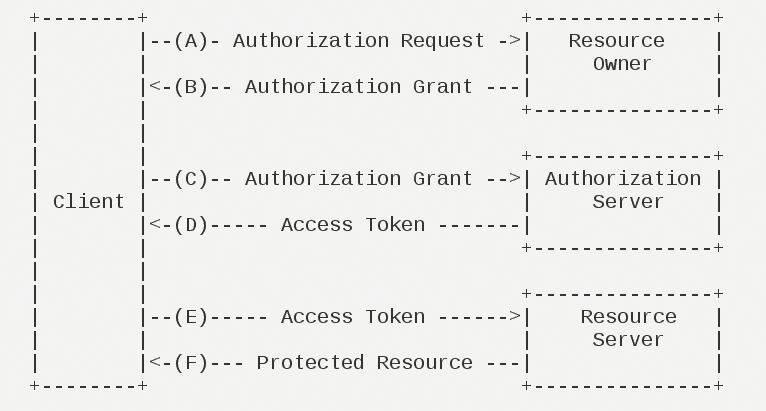
\includegraphics[width=14cm]{image/account/oauth.png}
    \fcaption{OAuth 2.0运行流程}
\end{center}
用户登出时,系统会将其重定向到Accounts9的页面,提示用户将Accounts9下线。

\subsection{访问权限控制}
一期工程中虽然区分了学生和管理员两类用户,但其区别仅仅体现在登陆后进入到不同的界面,对系统之后的运行过程中的用户访问权限并没有进行检查,例如学生可以通过修改URL地址栏而进入到管理员端。二期工程修复了这一问题,对于学生和管理员,通过核查authority域阻止权限非法的操作。此外,在涉及到与项目有关的操作时,也会在数据库中检查该项目id是否属于当前用户。

\subsection{同一账户多次登陆}
对于同一个浏览器,允许相同的账户多次登陆,均可以正常操作,且由于浏览器的本地缓存,再次访问实验平台时会跳过登陆界面,直接进入主页面。当用户登出时,此次会话的全部状态信息会被清空,此时若当前浏览器还存在该账户的其他登陆,则其下一步操作会跳转到登陆界面。

对于不同的浏览器,新的登陆会使前一次的登陆状态无效。即若用户用另一个浏览器再次登陆实验平台时,在前一个浏览器中的任何操作均会使会话的状态信息清空,从而跳转到登陆界面。这一机制是通过Accounts9返回的access token实现的,系统会用新的access token覆盖掉数据库中原有的该账户的access token,这样第一次登陆时获得的access token与服务器当前存储的access token就会失配。
\documentclass{article}
\usepackage{CJKutf8}
\usepackage{indentfirst}
\begin{document}
\begin{CJK}{UTF8}{gbsn}
\CJKindent
\section{用户端功能}

\par用户端功能主要分为电路拖拽编辑、VHDL代码编辑、项目信息显示、提交作业四大部分。本工程在第一期工程的基础上重构了整个电路拖拽编辑的架构、添加了提交作业的功能,并在仿真与VHDL代码编辑方面修改了若干bug,增加了部分新特性,使用户体验更佳。

\subsection{电路拖拽编辑}
    \par本项目中使用了更为成熟的Draw2D框架来代替一期工程中的Konva.js,并在原本在线拖拽搭建电路的基础上,添加了实时仿真、撤销操作等功能。
    \par下面介绍各个部件的实现细节:
\subsubsection{背景画布}
    \par背景画布以draw2D.Canvas为基类,使用了draw2D库中自带的多个policy(也即特性),并进行了修改以满足电路编辑需求。
    \par使用的policy列表如下:
    \begin{table}[!h]
    \begin{tabular}{|l|l|}
    \hline
    policy名字 & policy作用 \\
    \hline
    DropInterceptorPolicy & 接受Droppable对象 \\
    \hline
    DragConnectionCreatePolicy & 允许通过拖拽连接点产生连线 \\
    \hline
    OrthogonalConnectionCreatePolicy & 允许通过点击连接点产生连线 \\
    \hline
    CoronaDecorationPolicy & 鼠标接近时显示并高亮连接点,否则隐藏 \\
    \hline
    ShowGridEditPolicy & 在背景上显示网格,方便编辑与观察 \\
    \hline
    SnapToGeometryEditPolicy & 自动对齐部件 \\
    \hline
    SnapToCenterEditPolicy & 自动对齐部件 \\
    \hline
    SnapToInBetweenEditPolicy & 自动对齐部件 \\
    \hline
    EditEditPolicy & 编辑模式下使用,允许用户修改电路图 \\
    \hline
    SimulationEditPolicy & 实时仿真模式下使用,只允许用户查看电路图 \\
    \hline

    \end{tabular}
    \caption{policy列表}
    \end{table}

    \par为了方便用户使用,我们还使用了mousetrap库来捕获用户的按键输入,以提供快捷键功能。目前支持用户使用上下左右
    键移动画布与使用delete键删除元件。

\subsubsection{拖拽与缩放}
    \par用户可以通过shift+鼠标拖拽的方式来移动画布。上文中提到的两个EditPolicy中都添加了对shift按键的处理,在捕获到事件后,画布会随着鼠标的移动调整自身与网页的相对位置。
    \par同时,用户可以依靠画布右下角的缩放按钮来调整画布大小。由于Draw2d框架中自带setZoom方法用来调整背景画布的缩放与getZoom方法用来获取当前缩放,程序中只需要分别调用这些接口即可。
    \begin{table}[!h]
    \begin{tabular}{|l|l|l|}
    \hline
    按键 & 效果 & 代码段 \\
    \hline
    + & 放大画布及元件 & setZoom(this.getZoom()*1.2) \\
    \hline
    - & 缩小画布及元件 & setZoom(this.getZoom()*0.8) \\
    \hline
    100\% & 恢复原缩放 & setZoom(1.0) \\
    \hline
    \end{tabular}
    \caption{缩放相关函数}
    \end{table}

\subsubsection{元件}
    \par此次工程中的元件包含数字电路实验中的所有实验芯片及Vcc、GND、七段数码管、2-10进制转换器。所有芯片继承自draw2d.SetFigure,输入端使用DecoratedInputPort,输出端使用普通Port,标签为"output"。输入输出端只能接另一种端口,同种端口内部互联时网页会自动阻止操作。
    \par每个元件包含以下自定义属性及方法:
    \begin{table}[!h]
    \begin{tabular}{|l|l|}
    \hline
    名称 & 描述 \\
    \hline
    name & 芯片名称 \\
    \hline
    note & 芯片功能描述 \\
    \hline
    tagForWave & 元件标签,由用户搭建电路时编辑 \\
    \hline
    calculate & 实时仿真时每一个周期计算步骤\\
    \hline
    \end{tabular}
    \caption{元件参数及接口}
    \end{table}

    \par一个元件示例:
    \begin{table}[!h]
    \begin{tabular}{|l|l|}
    \hline
    名称 & 内容 \\
    \hline
    name & 74LS00 \\
    \hline
    note & "Y = not (A and B)" \\
    \hline
    calculate & Y1.setValue(!(A1.getValue() \&\& B1.getValue())); (其他端口同理) \\
    \hline
    \end{tabular}
    \caption{74LS00相关参数}
    \end{table}

    \par实际生成代码时,开关、50Hz脉冲等元件会被视为输入端口,小灯泡、七段数码管会被视为输出端口。
    \par元件列表在网页上会以画布外的悬浮列表形式显示,分为输入、输出与芯片三个部分,点击相应类别标题可以收起或弹出元件列表。当点击某一具体元件时,会生成一个带有元件类别信息的draw2d\_droppable对象,拖拽该对象进画布会触发画布的onDrop事件,进而在画布对应位置生成元件。
    \par每个元件的剩余数量会在元件列表中显示,onDrop事件会检查并修改剩余数量,并更新网页;删除元件时,同样会修改剩余数量,更新网页。

\subsubsection{标签}
    \par为了生成与电路图对应的VHDL代码用来仿真,每一个输入输出端口需要有唯一的标识符,也即标签。程序中通过jQuery的右键菜单功能允许用户右键点击元件来添加标签,或右击标签来删除标签。
    \par标签功能通过修改draw2d中的LabelInplaceEditor,自定义类AnotherLabelInPlaceEditor实现,支持修改和拖拽标签。
    \par接口:
    \begin{table}[!h]
    \begin{tabular}{|l|l|}
    \hline
    名称 & 内容 \\
    \hline
    commit & 修改完毕后提交修改内容 \\
    \hline
    cancel & 放弃修改内容 \\
    \hline
    \end{tabular}
    \caption{标签接口}
    \end{table}
    \par整个程序会维护一个已使用的名字集合,创建输入输出元件时默认命名为inx,outx(x为该类型元件总数量)。当用户试图修改标签或为其他元件添加新标签时,程序会检查以下三点合法性:
    \par1.通过正则表达式检查该名字是否符合VHDL命名规范,是否过长或为空;
    \par2.通过正则表达式检查该名字是否为VHDL保留字;
    \par3.检查是否与其他元件重名。
    \par如果不符合要求,程序会弹出对话框显示对应错误信息并取消修改,否则接受修改。此外,输入输出元件上的标签有特殊的标记,删除这些标签时网页会发出提示并拒绝修改,其他标签则可正常删除。
    \par每个标签上都安装了一个listener,会在标签的commit事件触发后修改相连接元件的tagForWave属性,供生成代码模块确定其名字。
    
\subsubsection{撤销与重做}
    \par二期工程中添加了撤销与重做的功能,当用户对之前做的操作不满意时,可以点击工具栏上的按钮来进行撤销与重做操作。
    \par Draw2d框架中自带了CommandStack功能,可以以栈的方式记录物体的添加、删除与移动操作,这部分解决了撤销的需求,但关联的属性仅限于画布基类内部,无法将元件剩余数量、元件名字同步更改。为此,我们改写了commandStack的stackChanged事件,在事件内部另外处理这些变更。具体处理的变更有:
    \par1.撤销元件的删除/添加操作时,修改元件剩余数量;
    \par2.撤销对标签的编辑时,修改相应元件的tagForWave属性;
    \par3.撤销生成/删除标签时,修改已用过的标签名集合。
    \par4.撤销栈或重做栈为空时,将对应按键设为灰色不可用状态。

\subsubsection{实时仿真}
    \par本工程支持实时仿真功能,实时仿真周期可通过工具栏中的滑动条调节。在仿真时,会根据每根导线上电平的高低决定导线的不同颜色,方便用户观察。
    \par具体实现思路为为每一个端口记录0/1值,对应低电平与高电平。每一个仿真时间点内,遍历所有导线,将输出端的值赋给输入端,然后根据元件的calculate函数计算出每一个输出端口的新值,如此循环。
    \par仿真开始与结束时的具体操作:
    \par仿真开始:使用SimulationEditPolicy,隐藏所有端口,将所有端口值初始化为0,开始循环仿真;
    \par仿真结束:使用EditEditPolicy,保留端口值。

\subsubsection{波形编辑}
    \par波形编辑部分使用外部库dygraph实现。在点击编辑波形按钮时,会自动读取电路图内容,提取输入端口标签名,生成对应编辑界面。用户修改电路图或标签名时,波形编辑器会相应发生变化。在波形编辑时(过长输入端口名字会被隐藏),用户可以通过拖拽或生成周期波形设置输入端口的激励值,或是设置总仿真时间。如果对波形显示不满意,还可以调整缩放比例,以取得更佳观察效果。
    \par接口如下:
    \begin{table}[!h]
    \begin{tabular}{|l|l|}
    \hline
    名称 & 说明 \\
    \hline
    downV4(event, g, context) & 鼠标按下事件,调用startEdit() \\
    \hline
    moveV4(event, g, context) & 鼠标移动事件,调用moveEdit() \\
    \hline
    upV4(event, g, context) & 鼠标松开事件,调用endEdit() \\
    \hline
    startEdit (event, g, context) & 记录端口名、开始位置等数据,开始编辑波形 \\
    \hline
    moveEdit (event, g, context) & 计算距离等数据,编辑波形 \\
    \hline
    endEdit(event, g, context) & 根据之前的数据,生成波形 \\
    \hline
    onclickStart() & 设置仿真时间 \\
    \hline
    onclickReset() & 将波形图重置 \\
    \hline
    onclickPlot() & 生成周期波形 \\
    \hline
    reloadJili(projectId) & 将波形信息上传给服务器 \\
    \hline
    \end{tabular}
    \caption{波形编辑接口}
    \end{table}

\subsubsection{杂项}
    \par导线使用draw2d.connection实现,采用InteractiveManhattanConnectionRouter,允许用户拖拽折点和导线段来微调导线。
    \par电路图与服务器间的交流使用draw2d中的writer.marshal实现,以json格式传递。在仿真与提交前,程序会自动将每一条导线的source和destination属性调整为输出端与输入端,方便后端程序生成代码。
    \par用户观看样例工程时,提交相关功能会被禁止;用户编辑作业工程时,允许用户提交电路图进行标准激励的测试。


\subsection{VHDL代码编辑}
    \par文本编辑器以开源的ace-editor为基础,可为VHDL代码实现高亮功能,并添加了一些其他功能。

\subsubsection{代码补全}
    \par程序支持自动补全VHDL关键字,如begin,architecture等,出现对应补全框时按回车即可补全,有效提高了用户编辑速度。该功能实现文件在/TextEditor/src-nonconflict/mode-vhdl.js中。

\subsubsection{代码折叠}
    \par过高代码量会影响用户调试,而代码折叠功能可以让用户将不需要的代码段收起,只显示需要的部分,提高调试效率。在case,if,begin-end语句旁会出现小箭头,点击该箭头即可收起或放出对应代码段。
    \par使用的函数有:
    \begin{table}[!h]
    \begin{tabular}{|l|l|l|}
    \hline
    名称 & 内容 & 返回值 \\
    \hline
    getFoldWidget(session,foldStyle,row) & 从对应行号开始进行折叠 & 折叠信息类 \\
    \hline
    getBeginEndBlock (session, row, column, matchSequence) & 搜索可折叠代码段并返回位置 & 代码段的开始与结束位置 \\
    \hline
    \end{tabular}
    \caption{代码折叠接口}
    \end{table}

\subsubsection{多文件}
    \par文件树部分采用开源库ez-filetree,可以显示文件列表,并支持新建、删除、重命名、打开、保存等功能。多标签编辑文件采用了开源项目hhEditor。
    \par使用的函数有:
    \begin{table}[!h]
    \begin{tabular}{|l|l|}
    \hline
    名称 & 内容  \\
    \hline
    getFileTree() & 向后端请求文件列表 \\
    \hline
    activate(file) & 打开对应文件并新建标签显示 \\
    \hline
    \end{tabular}
    \caption{多文件接口}
    \end{table}

\subsubsection{快捷键}
    \par程序支持多种快捷键:Ctrl+s可以保存文件或将新建文件保存新内容;双击文件标签可以进行重命名;ctrl+shift+d可以删除相应文件。

\subsubsection{编译信息}
    \par编译完成后,用户可以点击左下角显示本次编译信息,在单击具体错误信息时,还会打开出错文件并跳转到对应行。


\subsection{项目信息显示}
    \par用户登录时,网站会从后端获取该用户的所有项目列表,根据项目complieStatus属性的不同,显示会有一些差异:
    \begin{table}[!h]
    \begin{tabular}{|l|l|l|}
    \hline
    值 & 意义 & 颜色  \\
    \hline
    0 & 仿真通过 & 绿色 \\
    \hline
    1 & 尚未提交 & 蓝色 \\
    \hline
    2 & 编译成功但仿真失败 & 黄色 \\
    \hline
    3 & 编译失败 & 红色 \\
    \hline
    \end{tabular}
    \caption{多文件接口}
    \end{table}
    \par用户的自定义项目、作业项目、仅供观看的样例项目会分三个不同区块显示。

\subsubsection{提交作业}
    \par在上传完电路图信息与激励波形后,用户可以进行提交,进行modelsim仿真。对于作业项目,用户还可以提交自己的电路图,以教师设定的标准激励为输入进行仿真。
    \par用户可以在首页或相应工程的编辑页面中查看每一次提交的信息。对于自定义激励的提交,可以查看到编译信息,点击对应条目还可以查看每一个输入输出端口的波形信息,此界面同样使用外部库dygraph实现。
    \par但对于标准激励的提交,只显示最终得分,不显示编译信息及波形,以防止学生获得标准激励信息。
    \par此外,用户可以下载自定义激励提交的所有文件(包括电路VHDL代码、激励代码等),方便调试。

\end{CJK}
\end{document}
\section{管理员功能}
\section{测试}
    \setlength\parskip{0.3\baselineskip}
    \subsection{测试范围}
    考虑到项目上线的需要,测试部分除了单元测试以外还需要进行压力测试。前者主要确保用户的合法操作能得到预期的结果,非法的操作不至于影响项目运行安全或者访问无权限访问无权限访问的数据。
    \subsection{测试方法}
        \subsubsection{路由函数测试}
            \begin{itemize}
            \item \textbf{测试原理}
            
            \quad \quad 从用例的角度考虑,合理的测试方法是通过访问路由函数来模拟用户所有可能的操作。考虑到用户完全可以通过修改前端,甚至是直接使用脚本发出一些非法的请求。测试中http请求中的数据不应当完全依赖于前端的规定。亦即,对于每个路由函数,我们需要明确在它运行前可以确保什么一定是成立的,对于以外的东西需要在路由函数中检测;在运行后,我们需要明确在各种情况下什么东西一定会完成。

            \quad \quad 测试时主要采用判定覆盖的方法,对于主要的路由函数,同时采用了条件覆盖的方法。
        
            \item \textbf{代码内容}
            
            \quad \quad 路由函数在./routes目录下,对于主要的文件,我们使用 python 按照各个用例编写了脚本。脚本储存在./complex\_test/routes\_test中。在该目录下,同时存储了测试中需要用到的部分数据,例如vhdl代码和仿真文件。
            
            \quad \quad 在部分用例中,测试是从登录,创建项目开始,直到本用例的核心路由函数。对于每个用例,我们都给出了完全合法的访问的各种情况,以及非法的部分情况。后者主要是根据路由函数的代码以及常见的错误进行构造的。例如:我们假设用户试图通过各种奇怪的手段访问其它用户的项目,尽管阻止这种行为看似简单,但是仍然需要完善的用户管理和权限管理系统才能做到。
            
            \quad \quad 通过比对脚本中 http 请求的结果与预期的结果来判断是否通过了测试。由于报错时输出并没有统一格式,以及没有建立好测试代码与前端代码的联系,这种做法是缺乏可维护性的。测试过程中会将每个路由函数名,用例编号,测试结果逐个输出,通过即显示 true,未通过即显示 false。可以由此确定为通过的用例的位置。
            
            \quad \quad 在代码未完善之前,许多非法的操作是不可逆的,因而在路由函数测试结束后没有恢复系统本身的状态。相对应的,脚本中有变量test\_times,每次运行时加1,用于在每次测试中生成不同的项目名。
            
            \end{itemize}
        \subsubsection{压力测试}
            
            为了上线的需要,需要对项目进行压力测试。由于 Node.js 本身就具有高并发性的优势,故而用户的需要,即 60 人左右的并发规模是完全可以满足的。我们没有对并发性做出进一步的优化。但是仍然需要一定的测试进行检验。
            
            我们同样使用 python 脚本多线程访问,它们位于./complex\_test/stress\_test 目录下,主要包括两个文件,分别是针对两种主要的项目类型:文本编辑类型和拖拽类型进行测试。它们模拟了用户登录,创建项目,修改项目(上传文件,更改激励信号等),后端仿真,读取结果的过程。
            
            测试中发现同时的连续访问将导致项目无法正确地处理所有的请求,具体原因尚未找到。由于测试脚本中每个线程内部的请求是阻塞的,也就是说在下一个请求发出前,上一个请求的响应已经收到,推测是项目自身的原因,可能是在响应发出后,还有部分后续工作未完成,导致连续的接下来的访问无法得到正确结果。因而我们使用了一组变量来控制访问的间隔。结果将在下文详述
    \subsection{测试结果}
        \subsubsection{路由函数测试结果}
            在测试过程中发现了许多 bug,它们在代码中的相应位置都有注释。这些问题目前都已经被修复。
        \subsubsection{压力测试结果}
            这部分结果是项目尚未部署到服务器上时测试的,我们模拟的是最复杂的情况,即期末考试的完整流程,并发规模为 60。但是项目无法正确地处理同时的 60 个线程访问,在这种情况下只有约 20\% 的项目能从始自终完全正确地处理。要完全正确地处理,需要两个条件,单一线程的某些相邻请求之间需要一定的间隔(主要是创建项目后需要等待约 0.2 秒),多个线程的请求之间需要一定的间隔。对于后者,这里采取的办法是在每个线程的启动时,给予一定的时间间隔。从这个意义上而言,我们的项目并没有完全达到并发性的要求。但是,我们的项目能在20秒内处理完全部的工作。考虑到实际情况难以达到如此高密度的访问以及项目部署到服务器后的性能提升,我们的项目是能达到要求的。
\section{遇到的困难及解决方法}


\end{document}
% -----------------end------------------%
